%!TEX root = ../../thesis.tex
%!TEX enableSynctex = true
%*******************************************************************************
%****************************** Third Chapter **********************************
%*******************************************************************************
% **************************** Define Graphics Path **************************
\ifpdf
    \graphicspath{{Chapters/literature/Figs/Raster/}{Chapters/literature/Figs/PDF/}{Chapters/literature/Figs/}}
\else
    \graphicspath{{Chapters/literature/Figs/Vector/}{Chapters/Figs/}}
\fi

% Should include phototoxictiy http://www.nature.com/nmeth/journal/v14/n7/full/nmeth.4344.html

\chapter{Contemporary light-sheet technology}%:\\ \Large Correlating real-time viscoelastic changes with embryonic development}

Light sheet fluorescence microscopy (LSFM) is revolutionising the way in which complex, living biological samples can be imaged at high spatial and temporal resolution. %-
The technique deviates from conventional epi-fluorescence microscopy in that one illuminates the sample orthogonally to its detection.
The decoupling of illumination and excitation allows for the construction of light sheets whereby a single plane of interest is excited.  %CITE 14,15,16.
As such the technique offers optical sectioning capability comparable to a confocal microscope whilst still using a wide field detection system~\cite{siedentpf_uber_1903,voie_orthogonal-plane_1993,huisken_optical_2004-1}. %-
This garners two key advantages: firstly, as the plane of interest being detected is irradiated, the incident photon dosage is drastically reduced and so photo-toxicity to the sample is minimised.%-
This is in stark contrast to confocal imaging where signal is collected from a small voxel along the illumination axis whilst the entire sample is illuminated when recording a single image plane.
Secondly, wide field detection enables a significant temporal resolution increase in LSFM versus confocal.
For rapid volumetric imaging of complex organisms LSFM is becoming the technique of choice in developmental biology~\cite{keller_fast_2010,verveer_high-resolution_2007,mickoleit_high-resolution_2014,icha_using_2016,keller_visualizing_2015,ichikawa_live_2014}, plant science~\cite{wangenheim_rules_2016} and cell biology~\cite{capoulade_quantitative_2011,cella_zanacchi_live-cell_2011}.

The concept of orthogonal detection and illuminations dates back to 1903 when Zsigmondy and Siedentopf studied colloids in their \textit{Ultra-microscope}.
%who used a slit aperture and Sun light to image colloids in their \textit{Ultra-microscope} over in 1903 \cite{siedentpf_uber_1903}.
Technological advances in fluorescent dyes, labelling and digital image detection has permitted Voie~\emph{et~al}~\cite{voie_orthogonal-plane_1993}
to present the first light sheet fluorescence microscope in 1993.
%advances meant that in 1993, when Voie et al
%were able to present the first light sheet fluorescence microscope.
By 2004 Huisken~\emph{et al}~\cite{huisken_optical_2004-1}
demonstrated the potential of LSFM for \emph{in-vivo} imaging with cellular resolution.
Their Selective Plane Illumination Microscope (SPIM), seeded a rapid development in the LSFM field and is chosen here as an example to discuss the main concepts of LSFM.\@
\footnote{Design choices made here have heavily influenced the openSPIM project, an information toolkit found on the internet for constructing a LSFM}

%High quality LSFM is dependent on how well the illumination is generated.
%Huisken et al seminally used Gaussian laser emissions for the generation of their light sheets.
%Gaussian beams have a distinct trade-off when used in LSFM applications in that the thinner the light sheet designed the narrower the field of view; this can be seen in equation \eqref{eq:Guassian}, as $x$ increases or decreases (a movement away from the focus of the beam) the wider the beam gets.

%The Rayleigh length (or confocal parameter) in equation \eqref{eq:Rayleigh} is a metric for the distance over which a Gaussian beam still propagates as if it were parallel (neither converging nor diverging), for LSFM this is the distance over which it can be assumed the light sheet is of homogeneous thickness.

%Equation
%From equation \eqref{eq:Lorrentzian} g can be seen as having a dependence on the spot size or


\section{Generating Light Sheets}

\begin{itemize}
	\item[\checked] Optically  %\tick
	\item[\checked] Virtually
	\item[\checked] Volumetric Imaging
\end{itemize}	%Lightfield is instant 3D

\subsection{Light sheet generation}
\subsection{Optical Light sheet Generation}

%High quality LSFM is dependent on how well the illumination is generated.
Huisken~\emph{et~al} were seminal in their usage of Gaussian laser emissions for the generation of their light sheets despite Gaussian beams have a distinct trade-off when used in LSFM applications, in that the thinner the light sheet the narrower the usable field of view.
Equation~\eqref{eq:Guassian} models the Gaussian beam approximation where the full-width half-maximum ($\sqrt{\ln(2)}\omega(z)$) %\mynote[inline]{check maths}
increases as a Lorentzian when a distance $z$ away from the focal plane (Equation~\eqref{eq:Lorrentzian}).
The rate at which this occurs is dependent on the Rayleigh length in Equation~\eqref{eq:Rayleigh} which quantifies the trade-off.
The confocal parameter ($b=2z_R$) is a metric for the distance over which a Gaussian beam propagates as if it were parallel (neither converging nor diverging).
For LSFM this is the distance over which the light sheet can be assumed to be of homogeneous thickness.

Huisken also pioneered the use of a cylindrical lens to focus the Gaussian beam one dimensionally into a Gaussian light sheet.
The Gaussian nature of a beam's intensity for LSFM requires that the excitation beam is over expanded and later cropped by an aperture to create homogeneous illumination.
The procedure is optically lossy, but, laser intensity is typically in surplus for fluorescence microscopy techniques; a typical fluorescent sample needs $2\pm 1.5$ mW versus a low end diode laser emitting $100$ mW+.

%Huisken's SPIM had two distinct parts.
%The illumination path, which included a laser source beam expander to control the field of view of the light sheet and a  cylindrical lens to focus the beam into a thin sheet of light (Fig %FIGURE
%); and the detection path, which was similar to a standard widefield microscope including an objective lens, a tube lens and a camera.

\begin{align}
	I(r,z)    & = {I_0} {\left(\frac{\omega_0}{\omega{(z)}}\right)}^2 {e^{\frac{-2r^2}{\omega{(z)}^2}}\label{eq:Guassian}} \\
	\omega(z) & = \omega_0 \sqrt{1+\frac{z}{z_R}} \label{eq:Lorrentzian}                                                   \\
	z_R       & = \frac{\pi\omega_0^2}{\lambda} \label{eq:Rayleigh}
\end{align}

Where:\\
$z_R$ is the Rayleigh Length\\
$\omega_0$ is the spot of size of the beam.\\
$\lambda$ is the wavelength of light.\\

% Introduce Gaussian beam
% In cylindrical lens case laser light needs to be over expanded and cut to ensure a FOV homo

\subsection{Digital Light sheet Generation}

%Cylindrical lenses are bad because the sheet is highly coherent causing interference and more shadowing.
%A light-sheet crafted just using a cylindrical lens comes with it's own issues.
%Keller et al addressed
Keller~\emph{et~al}~\cite{keller_quantitative_2008} proposed sweeping a narrow laser beam through the sample to create a virtual light sheet.
This was achieved by oscillating galvanic mirrors at kHz frequencies, well over the Nyquist limit in comparison to the imaging acquisition rate~\cite{keller_quantitative_2008}.
To ensure a homogeneous illumination and distributed photon dosage a tele-centric f$\theta$ lens was used to convert beam angle optically from the scanning mirrors in to a linear position~\footnote{A practice borrowed from laser scanning microscopy.}.

Using DSLM instead of a cylindrical lens based system offers some key advantages.
Firstly, as the beam is scanned rather than stretched there can be no optical interference of coherent photons between neighboring regions, this reduces speckles and shadows.
Secondly, illumination intensity can be modulated such that structure can be superimposed on the sample giving the potential for super-resolution image improvement.
This resolution improvement has so far solely been experimentally demonstrated in the direction of the the scanning due to geometrical constraints~\cite{chen_lattice_2014}.

\subsection{Volumetric imaging}

The true power of light sheet microscopy becomes evident in its fast volumetric imaging capability.
Huisken's original SPIM required samples to be mechanically scanned through the static light sheet, potentially disturbing the sample depending on the speed of the scanning.
dSLM has the potential to subvert the static light sheet by using a second galvanometric mirror to move the light sheet relative to the static sample, the detection objective is then mounted on a high speed and precision axial translator and tuned to follow the light sheet.
Ideally piezoelectric actuators are used as their settling times are on the order of milliseconds providing speed and accuracy needed to match 100Hz cameras.
Of course, with dSLM, instead of the sample motion causing a disturbance a large objective local to the specimen is causing turbulence.
This was matched optically through the use of an electrically tunable lens~\cite{fahrbach_rapid_2013-1} that moves working distance of the detection objective.
%As such a new method was developed to achieve this optically, by using an electrically tunable lens to adjust the working distance of the detection objective.
This technique suffers from: fluorescent signal losses in the further four lenses and two mirror surfaces
\footnote{The mirrors are used to ensure the ETL is horizontal to gravity as further aberrations occur if the tunable surface is not entirely flat.
In essence two mirrors from the tunable light sheet could be removed by using mechanically deforming tunable lenses instead of electro wetting tunable lenses.}
($\sim 80$ percent signal retrieved); spherical aberration and is a more involved method as the system requires a non-linear calibration.


%Image of four configurations with details.
\section{Objective Arrangements}
\subsection{Single View}
%To ensure compatibility of Light sheet microscopes with biological mounting arranging.
Light-sheet microscopes are distinct in that two objectives are used orthogonally causing the technique to incompatible with most standard epi-fluorescent biological mounting practices.
Efforts have been made to make light sheet imaging more accepted through novel objective arrangements as well as new and intuitive mounting approaches.

\subsubsection{Horizontal Orientation}

\begin{itemize}
	\item[\checked]  Flat (openSPIM) open-SPIN diy-SPIM
				\item[\checked] MuVIEW\cite{swoger_multi-view_2007}%CITE"3060
	\item[\checked] Vert
	\item[\checked] V (diSPIM)
	\item[\checked] 60/30		Lattice Light Sheet and Objective Compatibility (Short section)
	\item[] Multi VIEW
\end{itemize}

%and the excitation objective illuminating through a clear window in the chamber.
Huisken~\emph{et~al.}, for instance, used two objectives in a horizontal configuration with a detection objective built into the sample chamber whilst the illuminating through a clear window.
This configuration was chosen so that a sample could be lowered into the system and, crucially, rotated without gravity causing registration errors when reconstructing the volume tomographically.
Rotational volumetric imaging also minimises shadows and improves image quality lost to scattering especially in thick \(>500 \mu m\) samples.
Mounting a sample from below and rotating produces the same result but requires a more sophisticated chamber design to contain the sample medium.
A horizontal geometry is vital also for plant biology as the objectives do not inhibit the plant's natural tendency to be upright~\cite{wangenheim_rules_2016}. %TODO CITE Stelzer
%Long working distance detection objectives have also been considered but the the lowered NA and

\subsubsection{Vertical Orientation}

An alternative to the Huisken's horizontal configuration is positioning the detection objective above the sample and illuminating from the side.
A vertical orientation is an attractive option as it can be compatible with commercial optical microscopes as well the chamber not requiring an inbuilt detection objective. %CITE 29 30
Both of these techniques can allow at  additional illumination objective, by offsetting the foci of the illumination objectives an overall more homogenous field of view can be created.


\subsubsection{(45 $^o$ Orientation)}

Shroff~\emph{et~al} then pioneered use of two objectives in a V configuration above the sample through iSPIM.\@
With choice objectives, adhered samples prepared with standard mounting procedures can be imaged in a petri-dish~\cite{kumar_dual-view_2014}.
%Other group then did the 45 degree inverted iSPIM.
%Shroff's diSPIM~\cite{kumar_dual-view_2014} then drastically improved axial resolution by imaging through both arms of the microscope.
%In doing so the axial resolution not collected through one arm is directly observed in the other.

%CITE 30 chick embryos

\begin{figure}
	\centering
	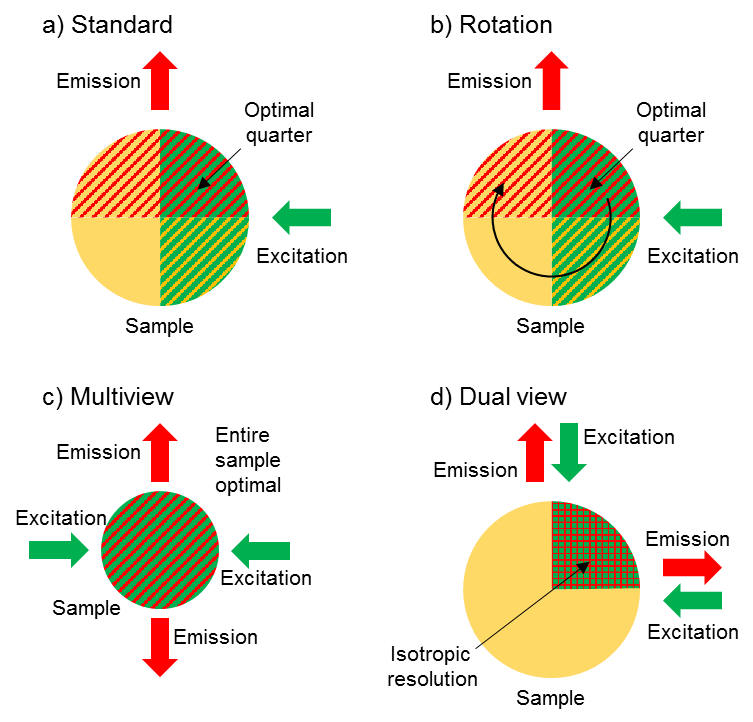
\includegraphics[width=\columnwidth]{spim_optimal_imaging.png}
	\caption{
	(a): The simple SPIM field of view – only a quarter of a sample has optimum illumination (green) and excitation (red).
	(b): by rotating a sample field of view can be quadrupled but at a cost in acquisition time.
	(c): By adding extra excitation and detection path the entire sample can be imaged without a rotation.
	(d): by making optical paths of a LSFM dual purpose a quadrant of a sample can be imaged from two orthogonal perspective and with correct image fusion achieve isotropic resolution.
	tod}
	\label{spim_optimal_imaging}
\end{figure}

\subsubsection{Optimal Orientation}

In a bid to maximise sample accessibility and numerical aperture, Betzig~\emph{et~al.}~\cite{chen_lattice_2014} commissioned a high NA (0.6) custom excitation objective to fit with their high NA (1.1) detection objective (Nikon CFI75).
In mounting the orthogonal pair at an angle such that they were flush so a flat surface, Betzig~\emph{et~al.} created the most unhindered sample mounting conditions realistically feasible using two objectives.
Tricks to circumvent objectives interfering with sample mounting are needed as high NA objectives are physically large.
%Numerical aperture depends on the $\sin$ of the collecting angle of light , intuitively this requires that the detecting objective to awkward in non-epifluorescence orientations. \mynote{reword}
%Moreover, the desire for high resolution images can cause spacial incompatibility between both objectives.
Moreover,  high NA objectives typically have short working distances and require both objectives to be close, and likely cause spacial incompatibilities even with the narrowest excitation objectives.
See figure~\ref{fig:objectivecompatibility} for a detailed comparison.

\begin{figure}
	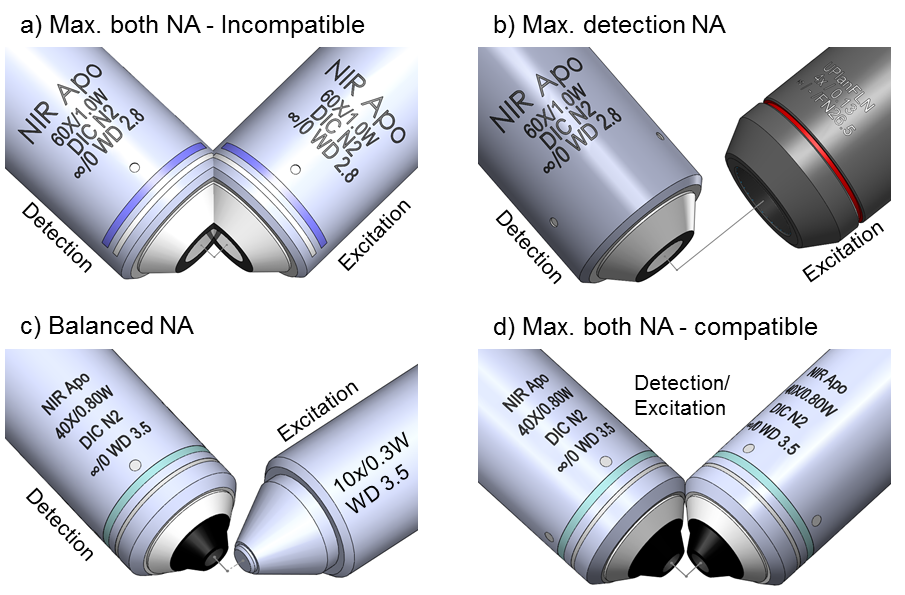
\includegraphics[width=\columnwidth]{objectivecompatibility}
	\label{fig:objectivecompatibility}
	\caption{}
\end{figure}

%Gaussian light sheet systems do not typically require such large NA excitation objectives meaning there are standard excitation objectives available.
%High NA objectives tend to have limited working distance and, in the orthogonal arrangements required for LSFM, have to be positioned very close to each other.

%suitably narrow such that flat substrates could be imaged.
%lattice light sheet style custom excitation.

%Gaussian beams don't need high NA excitation optics
%Large NA detection objectives have large collecting angles so a long working distance objective in desirable.


%subsection{MultiView}
\subsection{Multi-View}%\cite{swoger_multi-view_2007}

Shroff~\emph{et~al} introduced alternately imaging between each objective of the iSPIM in the form of the diSPIM~\cite{kumar_dual-view_2014}. %TODO Repeating myself
\footnote{This system is now a commercial light sheet solution provided by ASI.}
Axial resolution that would otherwise be lost to thick light sheets is recovered by switching the imaging and detection arms.
The two data sets captured by each camera are fused in post processing to provide near isotropic three dimensional resolution.
%\subsubsection{DualView}
%Shroff~\emph{et~al} not only pioneered the inverted SPIM (iSPIM) concept but also introduced alternately imaging between each objective in the form of diSPIM~\cite{kumar_dual-view_2014}. %TODO Repeating myself
%Axial resolution that would otherwise be lost to thick light sheets is recovered by switching the imaging and detection arms.
%The two data sets captured by each camera are fused in post processing.
%subsection{MuVU}
Where LSFM provides the most improvement over other techniques, such as in large, thick biological samples
%Where LSFM provides most improvement over other techniques
, scattering becomes significant both for excitation and emission light.
diSPIM however does not address inherent issues of scattering in thick samples, there is an \emph{optimal quarter} (see Figure~\ref{spim_optimal_imaging}) wherein excitation and emission photons are the least scattered.

Krzic~\emph{et~al} returned to the horizontal orientation of Huisken's SPIM, and chose their objectives wisely in MuVU-SPIM where two excitation and two detection objectives were packed around a hanging sample.
%cite objectives (Krzic et al. 2012)
MuVu can reach all regions of its sample, but it cannot dodge scattering limitations homogeneously.
%\subsection{Tomography}
To minimise gross scattering, sample rotation is necessary, of course acquiring volumes tomographically raises its own unique issues such as volume registration, rotational synchonisation and lengthy acquisition times.
Regardless, for large samples two objectives in Huiksen's original SPIM provide a cost effective robust volumetric imaging solution; with projects like the OpenSPIM have received significant acceptance and community attention.

\section{Single Objective Light Sheet Microscopy}

\begin{itemize}
	\item[\checked] Axial Plane \cite{li_axial_2014}
	\item[\checked] Oblique Plane \cite{dunsby_optically_2008}
	\item[\checked] Fibre SPIM \cite{ploschner_multimode_2015}
	\item[\checked] Mirrored Cuvette,
	\item[\checked] Confocal adaptor
\end{itemize}

Prior to refinements in objective positioning Dunsby conceptualised a system for single objective light sheet microscopy.
The advent of such systems could provide a plug-and-play light sheet experience on commercial microscope frames.
Dunsby proposed illuminating the sample using a high NA objective whereby the light sheet would illuminate at an oblique angle to the optical axis, the detected signal is then retrieved using the same objective~\cite{dunsby_optically_2008}.
Optically the sample is conjugated to a virtual position where a pair of objectives (excitation and detection) analyse the virtual sample in a conventional light sheet manner.
The technique suffers from optical technology, only when using a high NA objective can the system fully capture detection perpendicular to excitation.
Unfortunately, OPM is an involved technique as it requires that a standard light sheet microscope is constructed behind a further optical relay system.

Virtual sample manipulation is alluring as one can perform virtual manipulations that in are physically impossible.
Zhang et al~\cite{li_axial_2014} created their virtual sample using a similar relay system to Dunksby\emph{et~al}, but crucially they positioned an atomically flat mirror which precisely rotated their virtual sample by $90^o$.
In doing so they could illuminate the real sample along the optical axis and their virtual projection from the mirror was imaged directly onto a camera using a standard wide field configuration.

Using small mirrors near the sample is another viable, though more restrictive, approach to single objective LSFM.\@
Galland~\emph{et~al.} fabricated  micro-wells with $45^o$ micro-mirrors~\cite{galland_3d_2015}, converting any commercial scanning microscope into a light sheet microscope.
Leica produce a similar solution in the form of an objective adapter which holds two mirrored surfaces near the sample creating a similar effect.
Both techniques limit the size of the sample and their sectioning capability heavily depends on the quality of the mirrors used.

Ploschneret al.~attempted to minimise the size of the second objective rather than remove it.
By substituting the second objective for a multimode fibre~\cite{ploschner_multimode_2015} not only could they provide more access to their samples, but they could also embed their excitation source into their imaging chamber.
Assuming that a multi-mode fibre operates deterministically on an input light source, they were able to correct for the fibre using an SLM and further demonstrated the system's ability to produce exotic beam profiles.

%TODO cite scape

%subsection{Axial Plane}~\cite{li_axial_2014}
%subsection{Oblique Plane}~\cite{dunsby_optically_2008}
%subsection{Fibre SPIM}~\cite{ploschner_multimode_2015}

%Optical fibre transforms input light, can comepnsate and produce light sheets, bessel light sheets and lattice etc.
%Demonstrated in 0.25 NA fibre.
%Could use soft glass fibre to prove concept further.

%subsection{Confocal adaptor}

% High NA objectives require short working distances and large apetures
% An asymmetric pair
% an NA of 0.3 is needed to create a micron thick miaskla kzas
% Gaussian beam illumination requires low NA excitation and so assymetric pairs are ideal with a high NA detection being then possible (with a loss of axial resolution)
% Bessel illumination however requires high NA to construct the thin buy extended sheets and so are commcercially infeasible.
%Betzig et al. notabley used a custom excitation objective.
% Biological samples should be given room.

% Hence the ‘vertical at 90o’ approach can very attractive even if it cannot boast high NA excitation.
%Another limitation arises from geometrical compatibility of the objectives i.e. their opening angles cannot exceed 90o and the front lens radius of one objective should not exceed the working distance of the other objective.

%High NA detection and low NA excitation leads to high lateral resolution and low axial resolution.

\section{Illumination}

%\begin{itemize}
%	\item Variable Gaussian $\box$
%	\item Bessel\cite{gao_3d_2014}
%	\item Lattice light sheet.\cite{chen_lattice_2014}
%	\item Airy Beam $\box$
%	\item Multi-photon \checkmark~\cite{truong_deep_2011}
				%Comparison of Cost and Complexity?
%\end{itemize}

\subsection{Gaussian Techniques}
Illumination techniques have been proposed in a bid to circumvent the ubiquitous Gaussian beam extension versus thickness trade-off.
The most intuitive approach is accepting the loss of FOV produced by Gaussian illumination and moving the focus of this strip of high axial resolution light to different parts of the sample.
A final image can then be fused to achieve maximum axial resolution though with a direct cost for time of acquisition and photobleaching versus axial resolution, with an exceptionally high NA light sheet tending to becoming as slow and damaging as a confocal system.
\mynote{CITE Variable light-sheet.}
Fu~\emph{et~al.} proposed tiling multiple thin Gaussian light-sheets that are focally offset to create a similar tiling effect without the temporal loss~\cite{fu_imaging_2016}.
%The technique of tiled light-sheets was proposed recently whereby multiple thin Gaussian light-sheets are superimposed and focally offset to create a similar tiling effect without the temporal loss \cite{fu_imaging_2016}.
This effect was produced by using a Spatial Light Modulator whose hologram had superposed lens-like phase patterns superimposed.
This technique again suffers from the additional photo-dosage imparted by the undesirable lobes of the Gaussian beam, moreover these low resolution sections also contribute to fluorescent background reducing the net SNR of the system.
\subsection{Exotic Beams}
Species of exotic beam do exist which do not subscribe to classical Gaussian beam limitations.
%Airy beams, for instance, are non-diffracting, self healing beams.
% and I don't know anything about them over that Nikon use them?
Bessel beams are non-diffracting and self healing, meaning they reconstruct behind occlusions making them very desirable for light-sheet applications.
They can be optically constructed from either an axicon lens or a amplitude mask with a annual ring opening, the latter being inexpensive but the most optically lossy.
Unlike Gaussian optics their extension and thickness can be theoretically entirely decoupled, in practice a Bessel-Gauss beam only behaves over short distances \cite{gao_3d_2014} of up to $\sim 30\mu m$.
%\mynote[inline]{how short?}
% with the thickness being controlled by the outter-most radius and their extension
%Be beams both self heal,
Bessel beams however suffer from having multiple undesirable orders, the more ideal a Bessel beam is the more intensity is retained in its outer rings.
As such a singular scanned Bessel beam itself causes a significant background.
Betzig~\emph{et~al.}\cite{chen_lattice_2014} exploited these additional orders, they constructed multiple Bessel beams in the scanning plane by superimposing a sinusoidal amplitude pattern on to an annular amplitude mask.
In doing so their undesirable orders constructed to reinforce the zeroth orders of the parallel beams.
Finally they adjusted their now lattice light-sheet such that the outer orders above and below the scanning plane lay at minima in the detection point spread function reducing the net fluorescent axial background.
\subsubsection{Airy Beams}
Airy beams also self-heal similarly to Bessel beams but comparatively are more extended.
They are constructed using a coma-like phase pattern and exhibit characteristic a beam curvature.
Though they extend several fold further than Bessel beams, their curvature produces an asymmetric profile along the detection axis.
This is then required to be deconvolved in post processing.
Vettenburg~\emph{et~al}\cite{vettenburg_light-sheet_2014} demonstrated similar axial resolution improvement to Bessel beams whilst achieving a $\sim 3$ increase in field of view.
%It logically follows to create a lattice of Airy beams, this
%\mynote[inline]{TODO cite.}
%Airy beams are generated with a phase distribution resembling coma aberrations.
%These beams are characterised by longer extent compared to typically achievable Bessel beams (e.g. extension of 160 µm versus 60 µm for a Bessel beam with similar diameter) (Vettenburg et al. 2014).
%However, the Airy beams exhibit a curvature similar to coma aberrations and unsymmetrical higher orders in the beam radial profile, creating a PSF with characteristic unsymmetrical elongation along the detection axis (Morris et al. 2009). These can be corrected by deconvolving a measured stack using software methods.
%This can produce better resolution images with larger field of view compared to similarly deconvolved images obtained using Gaussian and Bessel beams (Vettenburg et al. 2014).
%However, this superiority over Bessel beams has only been demonstrated in comparison with the most basic Bessel beam setup, which does not compensate for higher orders of the Bessel beam distribution

\begin{figure*}
	\centering
	\label{fig:scatteringandshadowing}
	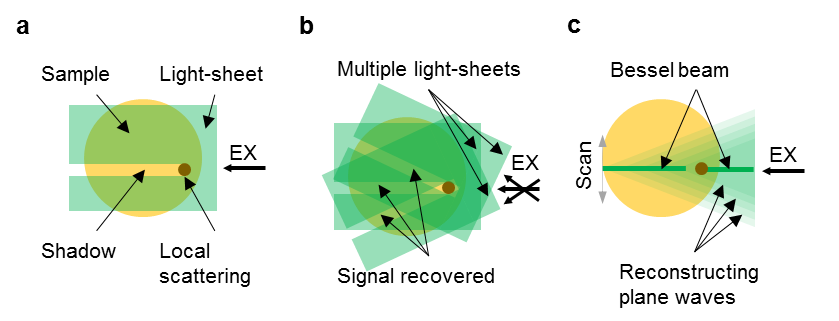
\includegraphics[width=\textwidth]{scatteringinlsfm}
\end{figure*}
\subsection{Thinner Beams}

Attempts to quantum mechanically narrow Gaussian Light sheets include using stimulated emission depletion and two photon emission (2P).
Using an addition laser to deplete, through stimulated emission (STED), out of plane fluorescence can narrow a Gaussian light sheet to $<1 \mu m$ \cite{friedrich_sted-spim:_2011}.
Two photon light sheet microscopy requires an excitation from two concomitant photons of cumulative energy sufficient bridge the required energy gap.
This requirement ensures that such excitation events are sufficiently rare and only occur where photon density is high.
%This requirement drastically reduces
%narrows the region in which fluorophores are likely to excite.
%By that two photons of cumulative energy sufficient to bridge the required energy gap, .
%By requiring that a fluorescent excitation only occurs when two photons of wavelength double that of the required energy gap,
In epi-fluorescent microscopes this occurs in the focal plane with the probability reducing quadratically along the imaging axis.
In light sheet microscopes this occurs at the axial centre of the light sheet making it much thinner than a comparable 1P excitation sheet.

%Exciting a
